\section{\textcolor{red}{Introduction}}\label{sec:intro}

\begin{wrapfigure}[19]{r}{0.525\textwidth} % <- 12 = approx. number of text lines to wrap
  \vspace{-50pt}                          % tighten top spacing (tweak as needed)
  \centering
  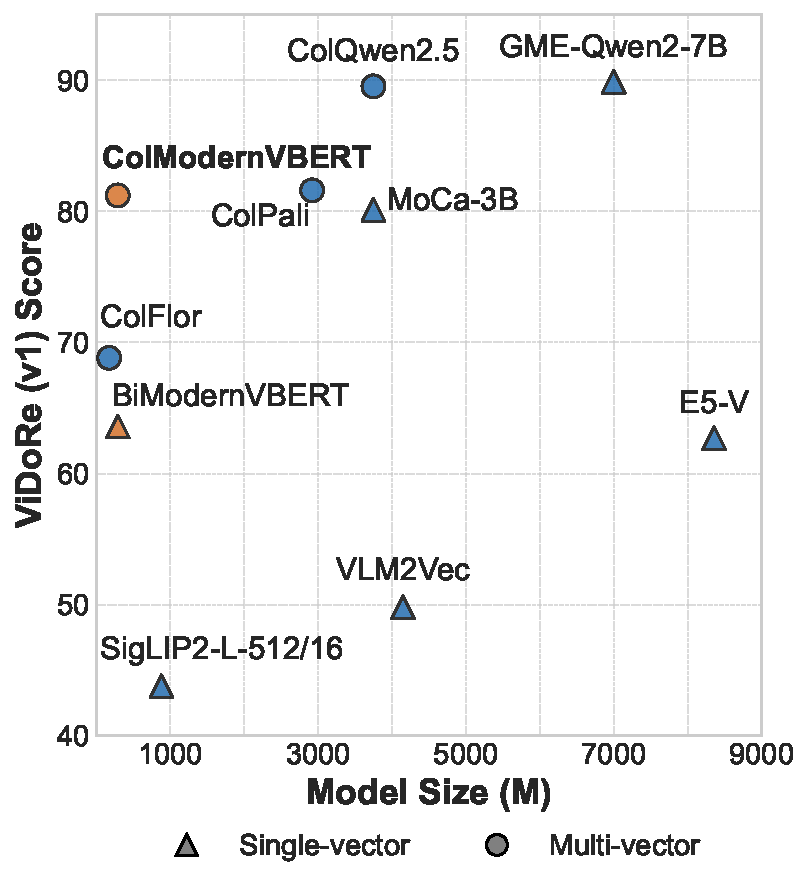
\includegraphics[width=0.88\linewidth]{figures/fig_1/pareto_large_models_ColModernVBERT_orange.pdf}
  \caption{\textbf{Pareto efficiency.} \colflagship{} outperforms models in its category on ViDoRe, achieving a leading performance-size tradeoff.
  }
  \label{fig:pareto_vidore}
  %\vspace{-10pt}                         % tighten bottom spacing (tweak as needed)
\end{wrapfigure}

% Context paragraph
% this is colpali's first paragraph, nice start point but to be modified. I think the reviewer is right in the sense that let's not overcomplicate the first paragraph. in the end its VDR so let's simply motivate it. @manu, c'est un draft fais toi plaisir, jen suis pas 100% convaincu de la forme mais j'aime le fond
% \textcolor{red}{Visual Document Retrieval (VDR) is a recently introduced alternative to text-based search systems, which, given a user query, consists in identifying relevant document pages within a large corpus by relying on their image screenshots rather than their pre-extracted textual content \citep{faysse2025colpaliefficientdocumentretrieval}. 
%Applications of Retrieval Augmented Generation (RAG) \citep{lewis_retrieval-augmented_2020} are ubiquitous in the industry, but remain bottlenecked by the quality of the first-stage retrieval system. To process documents such as PDFs, for many years, the standard approach was to extract the textual information of the documents--relying on OCR modules--and perform retrieval in the text space \citep{lin-byrne-2022-retrieval}.} Owing to the performance improvements enabled by generative vision–language models (VLMs), recent work has increasingly explored \textcolor{red}{operating in the vision space instead}, repurposing these models as multimodal encoders through extended contrastive post-training~\citep{ma2024unifyingmultimodalretrievaldocument,faysse2025colpaliefficientdocumentretrieval,jiang2025vlm2vectrainingvisionlanguagemodels}.

The ability to quickly locate specific information in vast document collections is a core building block of digital systems today, supporting use cases that range from web search and virtual assistants to enterprise knowledge management. Neural information retrieval (IR) models, and in particular dense retrievers, have become the de facto backbone of modern search systems thanks to their strong semantic matching capabilities and good scalability properties \citep{reimers_sentence-bert_2019, karpukhin_dense_2020, wang_text_2022}.  

This trend is amplified by the widespread adoption of Retrieval-Augmented Generation (RAG) \citep{lewis_retrieval-augmented_2020}, where a retriever is used to select a small set of relevant documents that condition a downstream generator. In such systems, the first-stage retrieval module is a well-known bottleneck: its recall directly upper-bounds the quality of the generated answers, while its latency and indexing costs partially drive the overall system efficiency \citep{lin-byrne-2022-retrieval}. As a result, improving document retrieval, especially for long, complex files such as PDFs, scientific articles, and reports, is a key lever for making industrial RAG deployments more accurate and cost-effective.
% \begin{wrapfigure}[24]{tr}{0.52\textwidth} % <- 12 = approx. number of text lines to wrap
%   \vspace{-5pt}                          % tighten top spacing (tweak as needed)
%   \centering
%   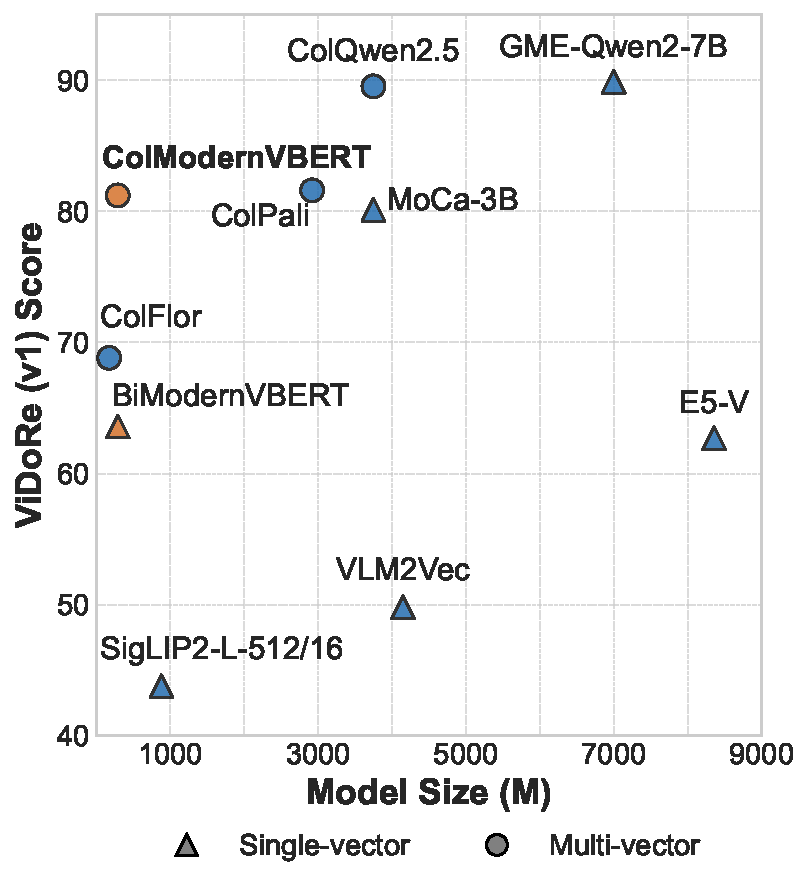
\includegraphics[width=\linewidth]{figures/fig_1/pareto_large_models_ColModernVBERT_orange.pdf}
%   \caption{\textbf{Pareto efficiency.} \colflagship{} outperforms models in its category on ViDoRe, achieving a leading performance-size tradeoff.
%   }
%   \label{fig:pareto_vidore}
%   %\vspace{-10pt}                         % tighten bottom spacing (tweak as needed)
% \end{wrapfigure}
\textbf{Visual Document Retrieval.} Historically, document retrieval in these settings has operated purely in the text space. To index PDFs or scans, practitioners first run heavy preprocessing pipelines that include Optical Character Recognition (OCR), layout analysis, and heuristic passage segmentation, before embedding the resulting text spans with a neural encoder. 
% \begin{wrapfigure}[23]{tr}{0.5\textwidth} % <- 12 = approx. number of text lines to wrap
%   \vspace{-5pt}                          % tighten top spacing (tweak as needed)
%   \centering
%   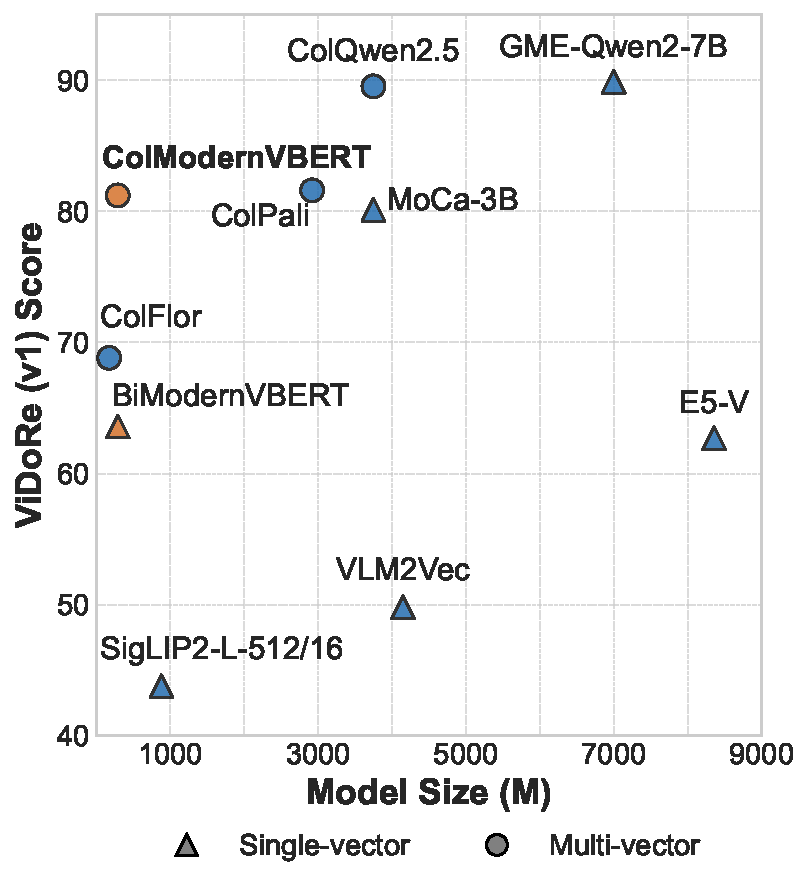
\includegraphics[width=\linewidth]{figures/fig_1/pareto_large_models_ColModernVBERT_orange.pdf}
%   \caption{\textbf{Pareto efficiency.} \colflagship{} outperforms models in its category on ViDoRe, achieving a leading performance-size tradeoff.
%   }
%   \label{fig:pareto_vidore}
%   %\vspace{-10pt}                         % tighten bottom spacing (tweak as needed)
% \end{wrapfigure}
This approach suffers from several limitations: OCR and layout parsing can be brittle and slow, complex visual elements such as tables, figures, and typography are often poorly captured, and any error or bias introduced during preprocessing is propagated to the retriever. % Recent work has shown that these multi-stage text pipelines can underutilize the rich visual structure of documents and leave significant performance on the table, especially in visually intensive domains \citep{faysse2025colpaliefficientdocumentretrieval}. 

\textit{Visual Document Retrieval} (VDR) has emerged as a compelling alternative to such text-based systems. Rather than indexing pre-extracted textual content, VDR models directly operate on page screenshots: given a user query, they retrieve relevant document pages by matching the query against image-based representations of the pages \citep{faysse2025colpaliefficientdocumentretrieval}. By bypassing OCR and layout parsing, VDR yields simpler end-to-end pipelines, significantly reduces indexing latency, and better exploits visual cues such as layout, figures, and fonts, while achieving strong performance on visually rich benchmarks like ViDoRe. 

\textbf{Limits of Generative VLM Repurposing.} Most current VDR systems are obtained by repurposing large generative vision–language decoders ~\citep{alayrac2022flamingovisuallanguagemodel} as retrieval encoders via post-hoc contrastive fine-tuning \citep{ma2024unifyingmultimodalretrievaldocument,faysse2025colpaliefficientdocumentretrieval,jiang2025vlm2vectrainingvisionlanguagemodels}. While cost-efficient, this design choice bottlenecks retrieval performance and efficiency: model sizes, attention patterns, image resolutions, and training objectives are designed for generative use cases rather than optimized for retrieval which has been shown in text models to be suboptimal \citep{lee2025nvembedimprovedtechniquestraining, gisserotboukhlef2025pretrainencodersmaskedlanguage}. Furthermore, scaling trends \citep{wei2022emergentabilitieslargelanguage} are less pronounced for embedding models; while correlated with model size, strong retrieval performance remains attainable with small models \citep{clavié2024bettermonolingualjapaneseretrievers}.

% Learning rich embeddings aligned between text and image modalities remains a central challenge in visual retrieval.
% A core challenge in visual retrieval is learning text–image embeddings that faithfully encode complex, multi-level semantics—from fine-grained details to high-level concepts.
% For many years, \emph{contrastive pre-training} of dual encoders, typically pairing a vision transformer (ViT)~\citep{dosovitskiy2021imageworth16x16words} with a text encoder, was the standard approach for generating cross-modal embeddings~\citep{radford2021learningtransferablevisualmodels,zhai2023sigmoidlosslanguageimage}. Owing to the performance improvements enabled by generative vision–language models (VLMs), recent work has increasingly explored repurposing these models as multimodal encoders through extended contrastive post-training~\citep{ma2024unifyingmultimodalretrievaldocument,faysse2025colpaliefficientdocumentretrieval,jiang2025vlm2vectrainingvisionlanguagemodels}. 






% While this approach capitalizes on the inherent capabilities of the backbone generative model to address complex visual tasks~\citep{alayrac2022flamingovisuallanguagemodel}, it is unclear whether the design decisions made for generative purposes hinder the models when repurposed for representation learning. 
% Typically, generative VLMs are built as vision extensions to Large Language Models designed for autoregressive generation, often with a focus on strong knowledge and reasoning skills.

% Typically, VLM-based encoders inherit the causal attention masks VLMs are trained with, which has been repeatedly shown to be suboptimal for embedding tasks~\citep{li2023generaltextembeddingsmultistage, behnamghader2024llm2veclargelanguagemodels,lee2025nvembedimprovedtechniquestraining,springer2025repetitionimproveslanguagemodel,gisserotboukhlef2025pretrainencodersmaskedlanguage}. 



% Another notable architectural property of contemporary VLMs is their high parameter counts. LLMs exhibit emergent abilities in reasoning and knowledge use as they grow in size \citep{wei2022emergentabilitieslargelanguage}, and most openly released decoders and their vision-augmented variants are at least several billion parameters. Interestingly, scaling trends are less pronounced for embedding models: while size remains a performance factor, compact encoders often almost rival the performance of much larger ones, indicating diminishing returns with additional parameters \citep{muennighoff_mteb_2022}. 
% Visual retrieval benchmarks such as ViDoRe and MIEB ~\citep{xiao2025miebmassiveimageembedding} are no exception, and model sizes within a same model family has been shown to deliver clear, but limited gains. Taken together, this 

% This suggests it is likely possible to achieve strong visual representation quality with relatively small, well-trained models, especially leveraging late interaction methods \citep{clavié2024bettermonolingualjapaneseretrievers}.



% What are we doing?
% \manu{Important not to be redundant with contributions detailed later on. --> In this paper, we opt to build document retriever models from the ground up, freeing ourselves from the constraints of strating from repurposed VLMs. Our contributions are the following:}
% \noindent\textbf{Revisiting Design Decisions in VLM Decoder Embedder Models.} 
% \manu{would be nice to introduce a bit more about the fact we are conducting controlled ablations. somethikgn along the line of - principled ablatioons have been done for vision models, for text models but not for vlms which are recent. this paper fills the gap. One thing we could put some emphasis on is how we "selected" the modality alignement mix to particularly be interesting for document retrieval (whether this is true or false, we make it sound like that. another key point is modality transfer for contratsive which is a cool "princiupled"result }
Recent papers and model releases in the visual retrieval space have claimed performance improvements by scaling the amount of contrastive data and the compute budget \citep{zhang2025gmeimprovinguniversalmultimodal, xu2025llamanemoretrievercolembedtopperforming}, modifying the attention mask \citep{chen2025mocamodalityawarecontinualpretraining}, increasing image resolutions \citep{cohere_introducing_2024} or by introducing more diverse tasks and data sources \citep{jiang2025vlm2vectrainingvisionlanguagemodels}. %Furthermore, it remains unclear whether the performance gains offered by these models are due to improved image representation capabilies or rather are enabled by aligned text and visual latent spaces.

% In this work, we revisit the entire training pipeline for visual document retrieval through controlled experiments, identify key design factors for effective VDR (including attention masking, image resolution, modality alignment data regimes, and late-interaction–centric contrastive objectives), and introduce ModernVBERT, a compact 250M-parameter vision–language encoder that outperforms recent VDR models up to ten times larger on document retrieval tasks, while enabling efficient inference on cheap CPU hardware.


In this work, we attempt to centralize these efforts and systematically disentangle the impact of core design decisions in visual retriever training. 
% Through rigorous experimentation in controlled setups, starting from language model pretraining to multi-stage domain specific finetuning, we attempt to identify: \textit{What makes a visual retriever great?} 
% By systematically disentangle the impact of core design choices in visual retriever training. 
Through controlled experiments—ranging from language model pretraining to multi-stage, domain-specific fine-tuning, we aim to answer a central question:
% \anto{On ne fait pas vraiment de language model pretraining - non mais on conbtrole pour ca}

\begin{center}
\textit{Which design choices best boost performance in modern visual document retrievers?}
\end{center}

% In this work, we take a principled approach ourselves how to best train a visual encoder from the ground up - freeing ourselves from the constraints of starting from pretrained VLMs. Our contributions are the following:

% \noindent\textbf{Contribution 1.}\; We critically reassess the core assumptions in multimodal encoder design. Contrary to the prevailing view, \textit{our analyses show the main strength of VLM-based encoders is not better image embeddings, but stronger alignment between image and text token embeddings}. Through controlled experiments, we measure the role of alignment length, training duration, and cross-modality interactions. We show alignment effectiveness is task-dependent, and provide evidence that causal attention is suboptimal in visual document retrieval, especially with late interaction~\citep{khattab_colbert_2020,faysse2025colpaliefficientdocumentretrieval}. \manu{something about causal attention here would make sense maybe ?}

% \manu{Is this still a contribution ? do we want to back up these claims ? esp. if the claims are document leaning ?}
% \noindent\textbf{Contribution 2: \natcap{}.}\; Existing contrastive datasets consist mainly of web-collected image–caption pairs or image–label pairs. Yet these pairs are often either too general (generic captions) or too narrow (single labels), lacking the contextual richness available in backbone LMs. To address this, we introduce \natcap{}, a contextualized image–caption dataset. We synthetically generate captions from classification training sets by providing the model with the image, its label, and task metadata as context. Through dataset ablations, we show that \natcap{} can be particularly beneficial for zero-shot classification tasks.

% \noindent\textbf{Contribution 3: \flagship{}.}\; Building on these insights, we design and release \flagship{}, \paul{double check this} the first multimodal encoder that aligns a pretrained language model encoder with a CLIP vision tower through Masked Language Modeling (MLM) objective. \paul{check ce qui suit avec les resultats} Despite its modest size and low data regime \manu{why low data regime ? prefer something like modest training budget}, this encoder outperforms \manu{give scale} larger VLM-based models on document retrieval while remaining competitive on natural image benchmarks \manu{the competitive natiure of ilages is something we want to claim ?}. Our results demonstrate that strong, efficient vision encoders can be obtained without the excessive parameter counts and architectural limitations of repurposed generative VLMs.

%\noindent\textbf{Contribution 1.}\; We revisit core assumptions in visual retriever design, showing that token-level objectives—beyond coarse contrastive alignment—are main drivers of retrieval performance, and that beyond strong image features, overlooked gains lie in improved fine-grained image–text alignment. We further show that causal attention is suboptimal in document retrieval, with bidirectional masking offering clear improvements in multi-vector settings, and that other parameters such as image resolution data mixes should not be overlooked in the training pipeline.

\noindent\textbf{Contribution 1.}\; We revisit core assumptions in visual retriever design, showing that token-level training objectives benefit retrievers by strengthening image–text token alignment—rather than merely producing stronger image embeddings.
Our results indicate that causal attention is suboptimal in document retrieval, with bidirectional masking offering clear improvements in multi-vector settings, and that other parameters such as image resolution data mixes should not be overlooked in the training pipeline.

% \noindent\textbf{Contribution 1.}\; We revisit core assumptions in visual retriever design. 
% % Token-level objective improves visual document retrieval performance
% We observe that token-level objectives consistently enhance document retrieval performance, and that beyond the use of strong image features, early fusion models yield overlooked benefits through improved fine-grained image–text alignment.
% % Causal attention is suboptimal in visual document retrieval, bidirectional attention unlock full potential of late inetraction, and other parameters such as image resolution and data mixes should not be overlooked.
% We further show that causal attention is suboptimal in visual document retrieval, with bidirectional masking offering clear improvements, and that other parameters such as image resolution data mixes should not be overlooked in the training pipeline.

% \noindent\textbf{Contribution 1.}\; We revisit core assumptions in visual retriever design. Notably, we show that causal attention is suboptimal in multi-vector document retrieval, with bidirectional masking offering clear improvements as a counterpart. We further show that token-level objectives—beyond coarse contrastive alignment—are important drivers of retrieval performance, and that beyond strong image features, overlooked gains lie in improved fine-grained image–text alignment.

%We critically reassess the core assumptions in visual retriever design. 

%We show that token-level objectives are beneficial in document retrievers training, and that contrary to the prevailing view, the main strength of VLM-based encoders is not better image embeddings, but stronger alignment between image and text token embeddings due to this token-level training objective. 

%We provide evidence that \textit{causal attention is suboptimal for visual retrieval tasks, especially in multi-vector settings}. Like in generative tasks, we observe that visual document retrieval is resolution-sensitive, 

%and that a cooldown on high-resolution images during modality alignment can improve model performances in such tasks.

\noindent\textbf{Contribution 2: \flagship{}.}\; Building on these insights, we release \flagship{}, a small \flagshipparameters{} multimodal encoder that aligns a pretrained language encoder with a vision encoder through Masked Language Modeling (MLM) objective, and \colflagship{} a variant fine-tuned for document retrieval. Despite its modest size and limited training budget, \colflagship{} matches models 10x larger on standard visual document retrieval benchmarks, demonstrating the interest of designing a retrieval focused model from the ground up. 
% We publicly release the model, intermediate checkpoints, and the training code at \repo{}.
\textcolor{red}{We release the model, intermediate checkpoints, and the training code at \repo.}

% Our results demonstrate that performant vision retrievers can be obtained without the excessive parameter counts and architectural limitations of repurposed generative VLMs.

% \begin{figure}[ht]
%     \centering
%     \includegraphics[width=0.6\textwidth]{example-image.png}
%     \caption{\paul{TODO} \manu{This could also be a table about what the different ablations taught us (green checkmarks, red crosses. Pareto might be too childish}}
%     \label{fig:pareto_frontier}
% \end{figure}

% \begin{figure}[t]
%     \centering
%     \includegraphics[width=\linewidth]{figures/fig 1/vbert_visu_fig1.pdf}
%     \label{fig:schema_causal_bidir}
%     \caption{\paul{TODO}}
% \end{figure}

% \begin{figure}[t]
%     \centering
%     \includegraphics[width=0.5\linewidth]{figures/pareto_plot.pdf}
%     \label{fig:pareto}
%     \caption{\paul{TODO}}
% \end{figure}


% We show The primary advantage of modality alignment methods (MLM/CLM objectives) lies not in improved intrinsic image embeddings, but rather in their ability to project text and image tokens into a shared latent space. 
% On top of that many MODELS ARE CONTRASTIVELY UNDERTRAINED. IN FACT, IN MANY OFF THE SHELF MODELS, THE TRAINING WORSENS THE EMBEDDING CAPABILITIES WRT SIGLIP.  We argue the interest of VLMs as encoders mainly lie on tasks where complex alignment with natural language queries are key (document retrieval), and analyze the impact of scaling both the modality alignement and the contrastive training phase, showcasing much performance is still up for grabs by scaling the contrastive training. 

% IDENTIFY THE AREAS WHERE THEY OUTPERFORM SIGLIPS.

% \noindent\textbf{Contribution 2.}\; We revisit the debate between encoder-only and decoder-based architectures, providing empirical evidence that bidirectional encoders outperform causal decoders in embedding quality. Additionally, we show that the performance gap between decoders and encoders can be bridged through post-training decoders using masked language modeling (MLM) objectives, but emphasize that substantial training duration is necessary. This gap is particularly pronounced in late-interaction retrieval methods, which currently dominate document retrieval benchmarks, highlighting the critical role of bidirectional attention mechanisms.

% \smallskip
% \noindent\textbf{Generative VLMs as embedding models.}\;Recently, \emph{generative} vision–language models (VLMs) combine a pretrained image encoder together with a large autoregressive decoder to perform a wide variety of generative multimodal tasks.
% Researchers have begun to repurpose these VLMs by extracting the text model's hidden state, running contrastive pretraining, reporting state‑of‑the‑art (SOTA) numbers on emerging benchmarks, e.g.\ DSE, VLM2Vec on \textsc{MMEB}  and ViDoRe. To further boost retrieval performance in complex image retrieval (documents), ColPali has shown that the vision-text alignement at a token level that VLMs exhibit enable retrieval with a late interaction operation which match text query tokens to corresponding image patch tokens. 

% \smallskip
% \noindent\textbf{Do VLM decoders really improve the \emph{image} representation?}\;
% % Mention MIEB where best models remain contrastive
% Although these repurposed VLM embedding models showcase strong retrieval performance, especially on document retrieval and on tasks contained within their contrastive training sets, more comprehensive image embedding benchmarks such as MIEB tell a slightly different story. Across most natural image tasks, the best models remain dual encoders, and this is particularly true in settings without corresponding text vectors (typically image classification with fixed classes, clustering). In this work we question whether as commonly believed feeding image embeddings to a text models really enriches the image representation, or whether the text model just facilitates learning mappings between text and image parameters.  We also question the common design choices of leveraging a causal decoder for representation tasks, while for text embeddigns, bidirectional encoders have times and times agin shown to be superior. Building upon these insights, we make the following contributions:

% \noindent\textbf{Contribution 1.}
% % revisit the design choices behind VLM encoders
% % show constrastively trained models remain best for image represenations, and that MLM/CLM alignement mainly help project text and image tokens to a simimlar latent space 
% % argue that it is more importznt to scake contrastive training than anlignement or model size

% \noindent\textbf{Contribution 2.} %revisit encoder vs decoder debate and show bidirectoonal attention is best. Show that the gap can be bridged by post-training decoders with MLM but it needs to be long enough. Show the gap is particularly meaningful for late interaction models which are currently the top performaing models on document retrieval benchmarks.


% \noindent\textbf{Contribution 3.} 
% % Apply lessons and release a small yet strong vision encoder model specialized for document retrieval tasks in public, outperforming bigger models


% Collectively, our results suggest that future progress in multimodal retrieval should prioritize better interaction strategies and training objectives over merely scaling decoders, and that strong, efficient vision encoders remain within reach without sacrificing simplicity.



% \section{Introduction}
% % Intro on image representations / document retrieva using images

% \noindent\textbf{Using VLMs for representation learning.}
% % mention colpali, Document screenshot embedding (DSE, Ma 2024), vlm2vec

% \noindent\textbf{Gap.} 
% % While VLMs claim strong performance on MMEBN, Vidore whoch are retrieval benchjmaerk, heavy on complex text inputs, more extensive evaluations on MIEN show they underperform on most natural language tasks. Decoder vs encoder debate (cite work)


% \noindent\textbf{Contributions.}